\section{Application Management and Setup}
\label{sec:setup}

\subsection{Package Management}

A package management system or, simply, a package manager is a collection of software tools that automates the process of installing, upgrading, configuring, and removing software packages in an easier and comprehensive manner. 
The package management in WP3 YouPower development uses state of the art technologies as follows: 

\begin{itemize}
\item Npm\footnote{\url{https://www.npmjs.com/}}, a package manager for JS,  and the default mackage manager for the JS runtime enviroment Node.js\footnote{\url{https://nodejs.org/}}. 

\item Bower\footnote{\url{http://bower.io/}}, a package manager for the front-end development to keep track of and update the packages. 

\item Gulp\footnote{\url{http://gulpjs.com/}}, a toolkit that helps to automate tasks in the development work-flow. 

\end{itemize}

\subsection{Localhost Setup}

For development of the application, one can set up and start a localhost as follows: 

\begin{itemize}

\item First install Node.js\footnote{\url{https://nodejs.org/}}, Npm\footnote{\url{https://www.npmjs.com/}},
Gulp\footnote{\url{http://gulpjs.com/}},  GraphicsMagick\footnote{\url{http://www.graphicsmagick.org/}} and MongoDB\footnote{\url{https://www.mongodb.com/}} on the local machine if any of those are not already installed. 

\item Optional: install Git\footnote{\url{https://git-scm.com/}} for version control.

\item Clone/import the (front-end and back-end) source code from the GitHub repository\footnote{\url{https://github.com/CIVIS-project/YouPower}} to the local machine. The source has a file structure as shown in Figure~\ref{fig:files}. 

\item Navigate to the project root directory \textit{YouPower} (or another directory name chosen for the source location) on the local machine and install dependencies: 
\begin{lstlisting}
cd YouPower
npm install
\end{lstlisting}

\begin{figure}
\centering
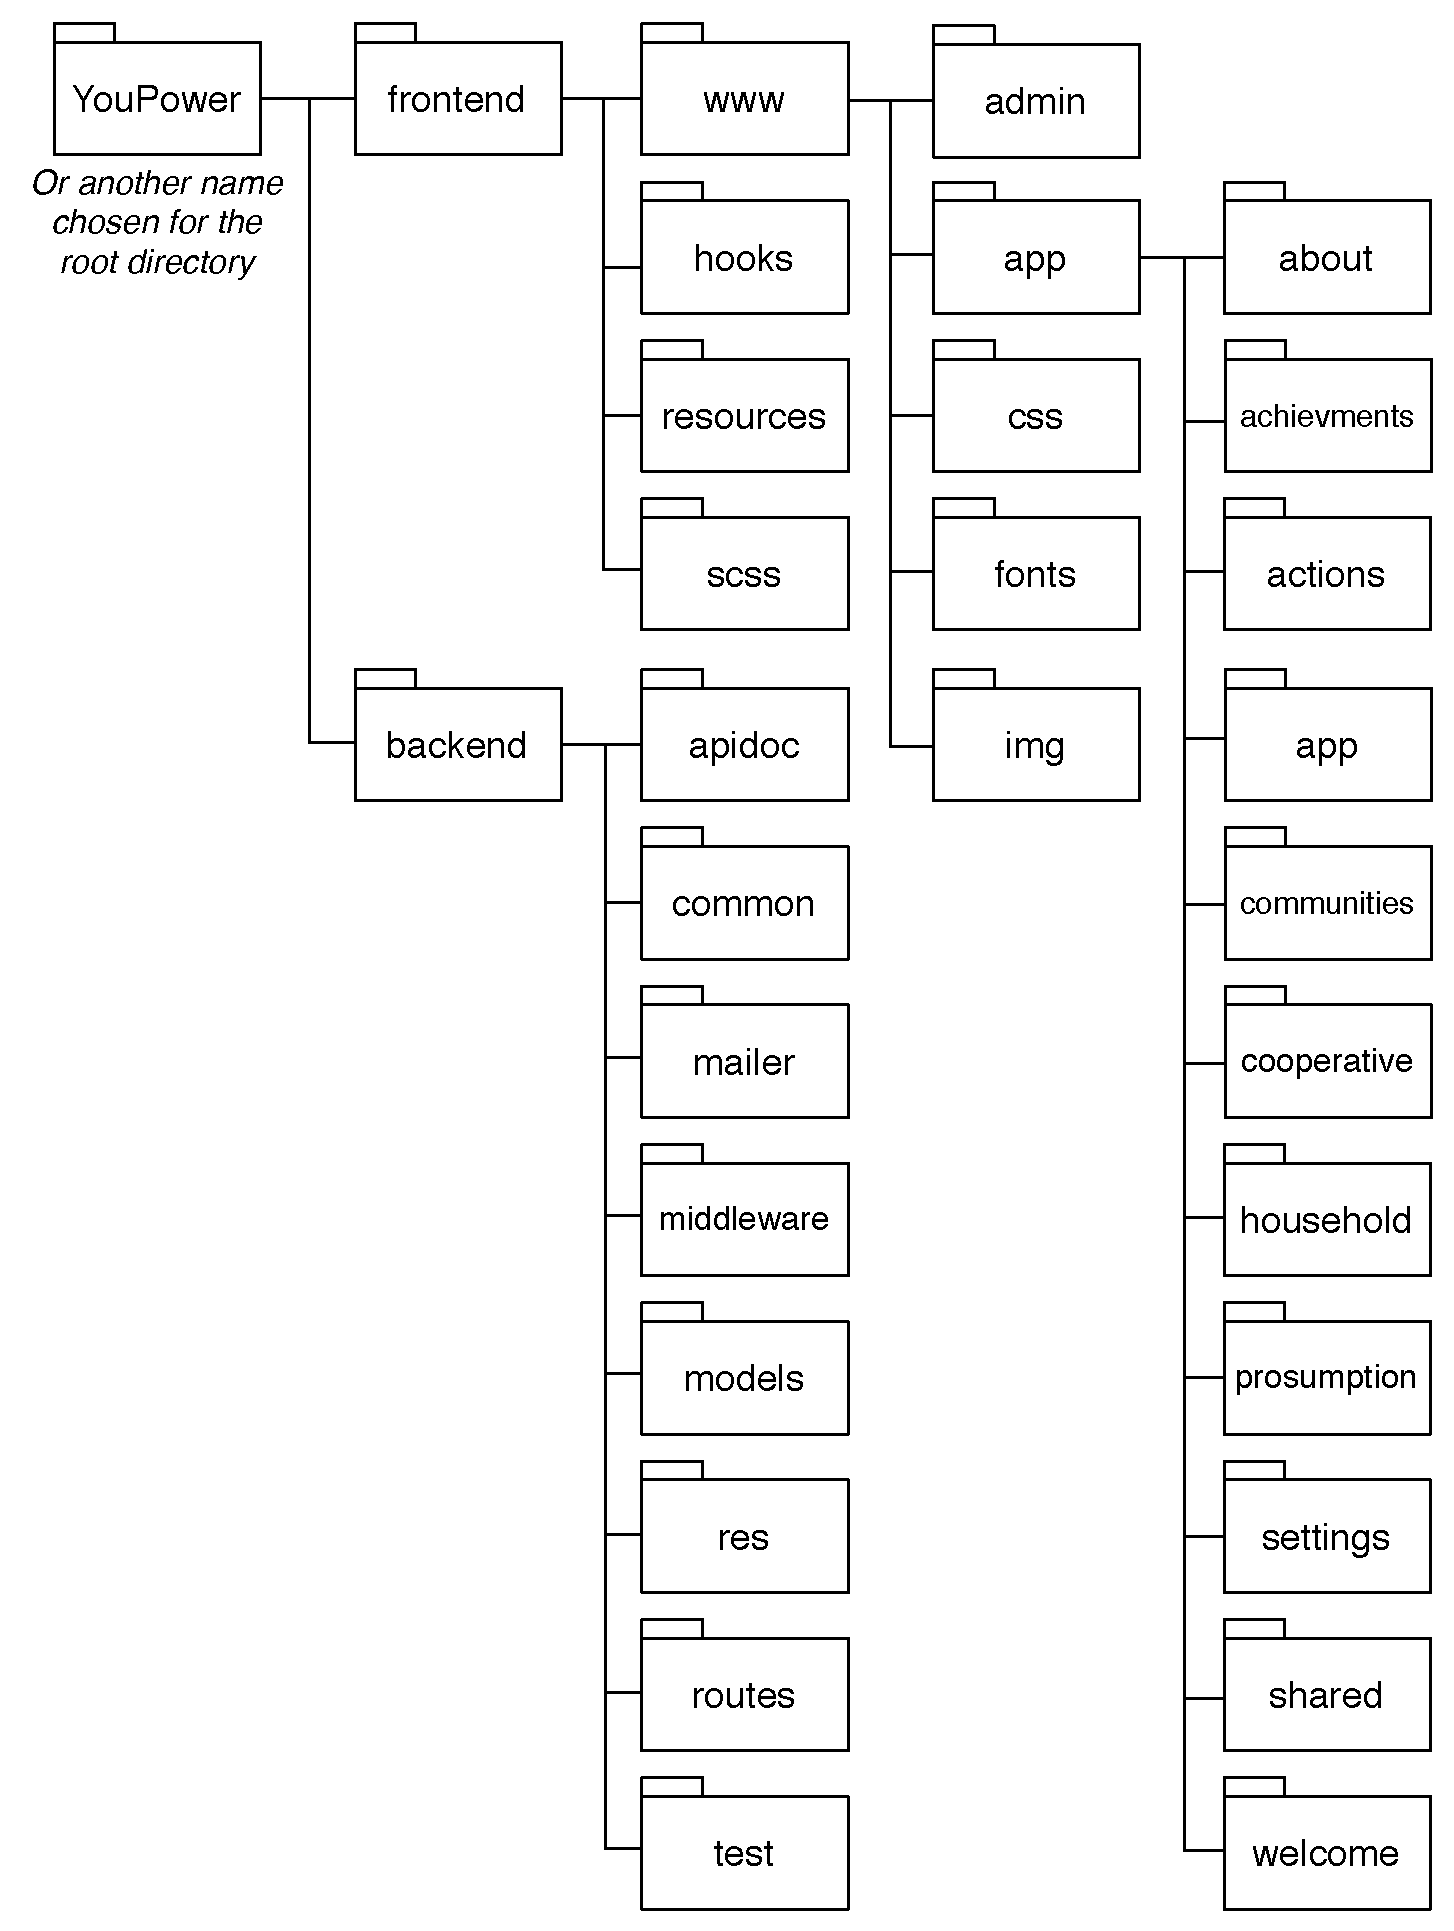
\includegraphics[width=0.9\linewidth]{img/files}
\caption{YouPower source code file structure}
\label{fig:files}
\end{figure}

\item Start MongoDB. The MongoDB installation and start process/commands are different on Linux/OSx/Windows machines. Please refer to the MongoDB manual\footnote{\url{https://docs.mongodb.com/manual/installation/\#tutorials}} for details.  

\item Start back-end server (1) with Npm start: 
\begin{lstlisting}
npm start
\end{lstlisting}
or (2) with Gulp: 
\begin{lstlisting}
gulp
\end{lstlisting}
When running the back-end with gulp, the back-end is restarted automatically each time when there is any change in \texttt{\small *.js} files. 

\item The REST API documentation is generated from inline code comments following the JSDoc specification\footnote{\url{http://apidocjs.com/}}. The documentation web page is generated/updated with:  
\begin{lstlisting}
gulp apidoc
\end{lstlisting}
The API documentation is then accessible at {\small\url{http://localhost:3000}}.

\item Navigate to the front-end directory \textit{YouPower/frontend}: 
\begin{lstlisting}
cd frontend                      
\end{lstlisting}

\item Install, build and start front-end server: 
\begin{lstlisting}
npm install -g bower cordova ionic        // install tools for build
npm install                          	   // install build dependencies
bower install										// install front-end dependencies
gulp													// build front-end
ionic serve											// start front-end server
\end{lstlisting}
The front-end is then accessible at {\small\url{http://localhost:8100}}.

\end{itemize} 

\subsection{Production Server Setup}

At the production server\footnote{\url{http://civis.tbm.tudelft.nl}}, WP3 uses \textit{Nginx}\footnote{\url{https://nginx.org/en/}} as the http and reservse proxy server. 
To set up Nginx, log on to the server machine and do the following steps: 

\begin{itemize}

\item Install Nginx if not already installed: 
\begin{lstlisting}
sudo apt-get remove apache2   	// remove the installed server e.g. apache
sudo apt-get install nginx 
\end{lstlisting}

\item Configure the reverse proxy rule by editing the file (e.g. on Debian/Ubuntu) : \\
\texttt{\small /etc/nginx/sites-enabled/default} \\
Add the following block in the file under the default  \texttt{\small location / \{...\} } block:
\begin{lstlisting}
location /api {
        proxy_pass      http://localhost:3000; 
}
\end{lstlisting}
This will proxy any requests beginning with \texttt{\small http://\{hostname\}/api} to the backend service running at port 3000. A similar block can be added for \texttt{\small location /apidoc} to expose the API documentation to the public.
\begin{lstlisting}
location /apidoc {
        proxy_pass      http://localhost:3000; 
}
\end{lstlisting}
The configuration file of the WP3 server can be found at GitHub\footnote{\url{https://github.com/CIVIS-project/YouPower-configs/blob/master/etc/nginx/sites-enabled/default}}. 
For more details about the configuration, refer to Nginx website\footnote{\url{https://nginx.org/en/}}. 

\item Change the root line in \texttt{\small /etc/nginx/sites-enabled/default} to the following:
\begin{lstlisting}
root /var/www/html;
\end{lstlisting}

\item Finally, restart the Nginx service to make all changes take effect:
\begin{lstlisting}
sudo service nginx restart
\end{lstlisting}
Nginx should then show a default page, and should proxy API requests to the back-end.

\end{itemize}

\noindent To set up the YouPower back-end on the production server, you can do the following steps: 

\begin{itemize}
\item Install the dependencies: 
\begin{lstlisting}
sudo apt-get install nodejs npm graphicsmagick git mongodb tmux 
\end{lstlisting}

\item Create a symbolic link to the Node location: 
\begin{lstlisting}
sudo ln -s /usr/bin/nodejs /usr/bin/node
\end{lstlisting}

\item It is preferable to do the next steps as a unprivileged user. On the TU Delft server we use user \textit{youpower}. In the following, we will use this username (and home directory) where needed. 
\begin{lstlisting}
sudo su youpower 									// change to the unprivileged user
cd  													// move to the home directory
\end{lstlisting}

\item Clone the (front-end and back-end) source code from the GitHub repository to the home directory, and install the dependencies:  
\begin{lstlisting}
git clone https://github.com/CIVIS-project/YouPower/
cd ~/YouPower
npm install 
\end{lstlisting}
Test running the back-end (it should stay running if everything works):
\begin{lstlisting}
npm start
\end{lstlisting}

\item To run the back-end as a Ubuntu update service, create a file (\texttt{\small /etc/init/youpower.conf}) as follows\footnote{\url{https://github.com/CIVIS-project/YouPower-configs/blob/master/etc/init/youpower.conf}}:
\begin{lstlisting}
description "YouPower backend"
author "CIVIS Project"

# When to start the service
start on runlevel [2345]

# When to stop the service
stop on runlevel [016]

# run as unprivileged user
setuid youpower

env HOME=/home/youpower
env FACEBOOK_APP_ID=<replaceme>
env FACEBOOK_APP_SECRET=<replaceme>
env FACEBOOK_CALLBACK_URL=<replaceme, e.g. https://app.civisproject.eu>

# Automatically restart process after crashed
respawn

# Start the process
exec /usr/bin/nodejs /home/youpower/YouPower/backend/app.js
\end{lstlisting}

Note: YouPower has Facebook login and share features which require permissions from Facebook. 
A registered application with \textit{Facebook Developers}\footnote{\url{https://developers.facebook.com}} obtains an App ID and an App Secret from Facebook, and can request for different types of permissions to access Facebook user data.  
This process is well documented on \url{https://developers.facebook.com}. If the Facebook features are used during development on the localhost, the  App ID and an App Secret are needed by the localhost as well. 

\item Start the back-end with:
\begin{lstlisting}
sudo service youpower start
\end{lstlisting}

\item To update a running back-end instance: 
\begin{lstlisting}
sudo su youpower     		// change to the youpower user
cd ~/YouPower 					// make sure you are in the correct directory
git pull							//	update to the latest master
gulp apidoc  					// update the apidocs 
sudo service youpower restart  		// restart the back-end
\end{lstlisting}
If the back-end doesn't start, find the upstart logs in:
\begin{lstlisting}
sudo tail -n30 /var/log/upstart/youpower.log
\end{lstlisting}

\end{itemize} 

\noindent To set up the YouPower front-end on the production server, you can do the following steps: 

\begin{itemize}

\item Clone the source code from the GitHub repository to the home directory if it is not updated: 
\begin{lstlisting}
git clone https://github.com/CIVIS-project/YouPower/ 
\end{lstlisting}

\item Navigate to the front-end directory, install and build the front-end: 
\begin{lstlisting}
cd ~/YouPower/frontend
sudo npm install -g bower cordova ionic gulp  // install tools for build
npm install                               //  install build dependencies
bower install                             // install clientside dependencies
gulp 									  				// build front-end
\end{lstlisting}
The built front-end should be in \texttt{\small $\sim$/YouPower/frontend/www}.

\item  Create a symlink to \texttt{\small index.html} called \texttt{\small frontend.html}:
\begin{lstlisting}
cd ~/YouPower/frontend/www
ln -s index.html frontend.html
\end{lstlisting}
This is needed because there is already an \texttt{\small index.html} on the web server, serving a web page of the YouPower project. In the next step, we configure Nginx to try the \texttt{\small frontend} directory as a fallback for missing files, and this wouldn't work if there are two \texttt{\small index.html} files. 

\item To make the \texttt{\small frontend} available to users, we configure Nginx to use this directory for missing files in the default path. Edit the file\footnote{\url{https://github.com/CIVIS-project/YouPower-configs/blob/master/etc/nginx/sites-enabled/default}} \texttt{\small /etc/nginx/sites-enabled/default}: change the default location's configuration block \texttt{\small location / \{...\}} by replacing
\begin{lstlisting}
try_files $uri $uri/ =404;
\end{lstlisting}
with 
\begin{lstlisting}
try_files $uri $uri/ @frontend;
\end{lstlisting} 

and add a \texttt{\small @frontend} block which looks as follows (please change the root path according to where the \texttt{\small frontend} directory is located):
\begin{lstlisting}
location @frontend {
        root /home/youpower/YouPower/frontend/www;
        try_files $uri $uri/ =404;
}
\end{lstlisting} 

So we end up with:

\begin{lstlisting}
location / {
        try_files $uri $uri/ @frontend;
}

location @frontend {
        root /home/youpower/YouPower/frontend/www;
        try_files $uri $uri/ =404;
}
\end{lstlisting} 

\item Restart Nginx server to reload the configuration:
\begin{lstlisting}
sudo service nginx restart
\end{lstlisting} 

\item To update the front-end:
\begin{lstlisting}
sudo su youpower                // change to the correct user
cd ~/YouPower/frontend
git pull
npm install                    // install missing build dependencies
bower install                  // install missing clientside dependencies
gulp                           // rebuild frontend
\end{lstlisting} 


\end{itemize}